\section{Polygon Class Reference}
\label{classPolygon}\index{Polygon@{Polygon}}
{\tt \#include $<$polygon.h$>$}

Inheritance diagram for Polygon::\begin{figure}[H]
\begin{center}
\leavevmode
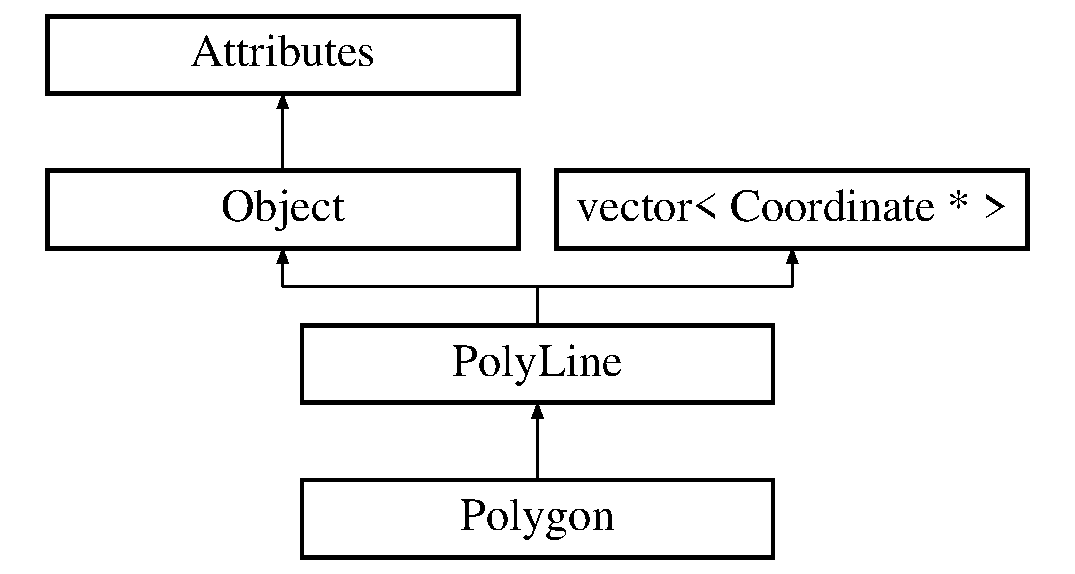
\includegraphics[height=4cm]{classPolygon}
\end{center}
\end{figure}
\subsection*{Public Methods}
\begin{CompactItemize}
\item 
{\bf Polygon} ()
\item 
{\bf Polygon} ({\bf Coordinate} $\ast$, {\bf Coordinate} $\ast$)
\item 
{\bf $\sim$Polygon} ()
\end{CompactItemize}


\subsection{Detailed Description}
This class handles polygons. This class is derived from {\bf Poly\-Line} {\rm (p.\,\pageref{classPolyLine})}. \begin{Desc}
\item[Author: ]\par
Anthony Liekens \end{Desc}




\subsection{Constructor \& Destructor Documentation}
\index{Polygon@{Polygon}!Polygon@{Polygon}}
\index{Polygon@{Polygon}!Polygon@{Polygon}}
\subsubsection{\setlength{\rightskip}{0pt plus 5cm}Polygon::Polygon ()}\label{classPolygon_a0}


\index{Polygon@{Polygon}!Polygon@{Polygon}}
\index{Polygon@{Polygon}!Polygon@{Polygon}}
\subsubsection{\setlength{\rightskip}{0pt plus 5cm}Polygon::Polygon ({\bf Coordinate} $\ast$, {\bf Coordinate} $\ast$)}\label{classPolygon_a1}


\index{Polygon@{Polygon}!~Polygon@{$\sim$Polygon}}
\index{~Polygon@{$\sim$Polygon}!Polygon@{Polygon}}
\subsubsection{\setlength{\rightskip}{0pt plus 5cm}Polygon::$\sim$Polygon ()}\label{classPolygon_a2}




The documentation for this class was generated from the following files:\begin{CompactItemize}
\item 
{\bf polygon.h}\item 
{\bf polygon.cpp}\end{CompactItemize}
